%% ma: L10-B24-0001
%% lop: 10
%% chuong: 8
%% bai: 24
%% dang: 10.24.1
%% loai: TLN
%% muc: VD
%% dap_an: "43"
%% nguon: "0. ĐỀ THAM KHẢO TN THPT 2025.pdf (D00), Phần III Câu 2"
%% kien_thuc: "Đồ thị có trọng số, chu trình Hamilton (không có trong mục lục sgk-kntt.yaml); cách giải cần liệt kê hoán vị (Lớp 10 Bài 24)"
%% ghi_chu: "Đề gốc: hình không xuất hiện ở trang đề (chỉ có ở trang lời giải), viết sai '4,B,C,D' thay cho A,B,C,D; đã sửa và dùng hình ở lời giải. Đáp án 43 đúng (kiểm bằng liệt kê 3 chu trình). Lớp 10 Bài 24 là vị trí tạm, giáo viên đã duyệt giữ câu"
%% trang_thai: chinh-thuc
\begin{ex}
Một trò chơi điện tử quy định như sau: Có $4$ trụ $A,B,C,D$ với số lượng các thử thách trên đường đi giữa các cặp trụ được mô tả trong hình bên. Người chơi xuất phát từ một trụ nào đó, đi qua tất cả các trụ còn lại, mỗi khi đi qua một trụ thì trụ đó sẽ bị phá hủy và không thể quay trở lại trụ đó nữa, nhưng người chơi vẫn phải trở về trụ ban đầu. Tổng số thử thách của đường đi thỏa mãn điều kiện trên nhận giá trị nhỏ nhất là bao nhiêu?
\begin{center}
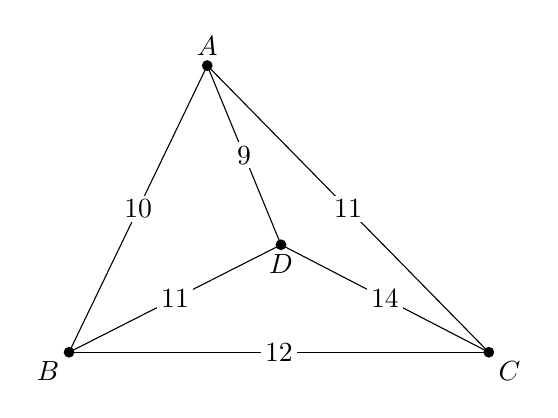
\begin{tikzpicture}[scale=1.3]
  \path (0,0) coordinate (B) (4.1,0) coordinate (C) (1.35,2.8) coordinate (A) (2.07,1.05) coordinate (D);
  \draw (A)--(B) node[midway,fill=white,inner sep=1.5pt]{$10$};
  \draw (A)--(C) node[midway,fill=white,inner sep=1.5pt]{$11$};
  \draw (A)--(D) node[midway,fill=white,inner sep=1.5pt]{$9$};
  \draw (B)--(C) node[midway,fill=white,inner sep=1.5pt]{$12$};
  \draw (B)--(D) node[midway,fill=white,inner sep=1.5pt]{$11$};
  \draw (D)--(C) node[midway,fill=white,inner sep=1.5pt]{$14$};
  \foreach \P in {A,B,C,D} \fill (\P) circle (1.5pt);
  \path (A) node[above]{$A$} (B) node[below left]{$B$} (C) node[below right]{$C$} (D) node[below]{$D$};
\end{tikzpicture}
\end{center}
\shortans{43}
\loigiai{Đường đi là một chu trình qua đủ $4$ đỉnh nên gồm $4$ cạnh, tức là bỏ đi hai cạnh không chung đỉnh. Tổng số thử thách của $6$ cạnh là $9+10+14+12+11+11=67$.
Bỏ $AD,BC$: $67-9-12=46$. Bỏ $AB,DC$: $67-10-14=43$. Bỏ $AC,BD$: $67-11-11=45$.
Vậy giá trị nhỏ nhất là $43$.}
\end{ex}
